\documentclass[xcolor=svgnames, compress]{beamer}
%\documentclass[compress,red]{beamer}

\mode<presentation>

\usepackage{amsmath}

\usepackage{ragged2e}


\usepackage{comment}
\usepackage{multirow}
\usepackage{amsmath, amssymb}
\usepackage{graphicx}
\usepackage{color}

\usepackage{xcolor}


%\usepackage{arydshln}
\usepackage{marvosym}

\usepackage{hyperref}


\usepackage{booktabs, tabu}

\usepackage{tikz}
\usetikzlibrary{arrows,shapes,trees}
\usetikzlibrary{matrix}
\usetikzlibrary{calc}
\usepackage{tabularx}

\usepackage{hhline}% http://ctan.org/pkg/hhline


%\includepackage{multimedia}

%\documentclass[draft]{beamer}
%\documentclass[compress]{beamer}
%\documentclass[xcolor=pst]{beamer}
%\usenavigationsymbolstemplate{}
%\setbeamertemplate{navigation symbols}{} 



\definecolor{oiB}{HTML}{569BBD}
\definecolor{oiB2}{HTML}{67A5C4}
\definecolor{oiB3}{HTML}{78AFCB}
\definecolor{oiB4}{HTML}{89B9D2}
\definecolor{oiB5}{HTML}{9AC3D9}
\definecolor{oiB6}{HTML}{ABCDE0}
\definecolor{oiB7}{HTML}{BCD7E7}
\definecolor{oiB8}{HTML}{CDE1EE}
\definecolor{oiB9}{HTML}{DEEBF5}
\definecolor{oiB10}{HTML}{EFF5FC}

\usetheme{UniversiteitAntwerpen}
%\usetheme{Ilmenau}
%\usetheme{Frankfurt}
%\usetheme{Amsterdam}
%\usetheme{Warsaw}


%\usetheme{Darmstadt}
%\useoutertheme{miniframes}
%\makeatletter
%  \beamer@compresstrue
%\makeatother



\setbeamercovered{transparent}


\useinnertheme{rounded}
\setbeamertemplate{items}[ball]
\setbeamertemplate{blocks}[rounded][shadow=true]
\setbeamertemplate{navigation symbols}{}
\setbeamercolor{normal text}{fg=Black}



\newtheorem{goal}{Goal}
\newtheorem{nt}{Note}

\newtheorem{axioms}{Axioms}
\newtheorem{rl}{Rule}

\newtheorem{prop}{}

\newtheorem{pmf}{Probability Mass Function}



\newenvironment{changemargin}[2]{%
\begin{list}{}{%
\setlength{\topsep}{0pt}%
\setlength{\leftmargin}{#1}%
\setlength{\rightmargin}{#2}%
\setlength{\listparindent}{\parindent}%
\setlength{\itemindent}{\parindent}%
\setlength{\parsep}{\parskip}%
}%
\item[]}{\end{list}}


\newcommand*\circled[1]{\tikz[baseline=(char.base)]{
            \node[shape=circle,draw,inner sep=2pt] (char) {#1};}}

\newcommand*\dash{\rotatebox{90}{\Kutline} }


\usepackage{array}
\newcolumntype{L}[1]{>{\raggedright\let\newline\\\arraybackslash\hspace{0pt}}m{#1}}
\newcolumntype{C}[1]{>{\centering\let\newline\\\arraybackslash\hspace{0pt}}m{#1}}
\newcolumntype{R}[1]{>{\raggedleft\let\newline\\\arraybackslash\hspace{0pt}}m{#1}}



\newcommand*\dashline{\rotatebox[origin=c]{90}{$\dabar@\dabar@\dabar@$}}



\DeclareRobustCommand{\rchi}{{\mathpalette\irchi\relax}}
\newcommand{\irchi}[2]{\raisebox{\depth}{$#2\chi$}}




%\setbeamertemplate{headline}{%
%\leavevmode%
%  \hbox{%
%    \begin{beamercolorbox}[wd=\paperwidth,ht=3.5ex,dp=12.125ex]{palette quaternary}%
%    \insertsectionnavigationhorizontal{\paperwidth}{}{\hskip0pt plus1filll}
%    \end{beamercolorbox}%
%  }
%}




\AtBeginSection[]
{
\begin{frame}<beamer>{Table of Contents}
   %\begin{frame}
        %\frametitle{Inhalts\"ubersicht}
        %\frametitle{Inhalts\"ubersicht}
	\small        
        \tableofcontents[currentsection,currentsubsection]
	\normalsize
   \end{frame}
}










\title{1. Introduction\\
\vspace*{-0.25cm}
{\normalsize{STAT*2060: Statistics for Business Decisions} } }
\author{Nishan Mudalige}
\institute{Department of Mathematics and Statistics\\
University of Guelph}
\date[STAT*2060F14]{Fall 2014}

\begin{document}

\small

%\frame{\titlepage}

\begin{frame}
\vspace{-2.0cm}
\maketitle
\end{frame}


\begin{frame}
\frametitle{Table of Contents}
\tableofcontents
\end{frame}


\section{Basics}



\subsection*{Basics}

\begin{frame}
\frametitle{Basics} 

%Recall from our overview:\\
%\hfill\\

\vspace{-0.50cm}
\begin{definition}[Statistics]
\justifying
Statistics is the science of collecting, classifying, summarizing, analyzing and interpreting data.
\end{definition}


\hfill\\
%\vspace{-0.3cm}

\begin{definition}[Descriptive Statistics]
\justifying
Numerical and graphical methods used to analyze, interpret and represent data.
\end{definition}


\hfill\\
%\vspace{-0.3cm}

\begin{definition}[Inferential Statistics]
\justifying
Use information from a sample to make generalizations about a population.
\end{definition}



\end{frame}




\section{Types of Data}

\subsection*{Types of Data}


\begin{frame}
\frametitle{Types of Data} 

\vspace{-0.25cm}

\begin{definition}[Quantitative data]
\justifying
Numerical data that can be measured.
\end{definition}

%\hfill\\

\begin{itemize}

\item	Examples:
	\begin{itemize}\justifying
	\item	Number of hours you studied this week
	\item	Distance from your house to the university
	\item Area (in ft$^{2}$ ) of the floor of a concourse
	\end{itemize}

\hfill\\

\item	Quantitative data can also be divided into:
	\begin{itemize}
	\item	Discrete data
	\item	Continuous data
	\end{itemize}
\end{itemize}

\end{frame}


\subsection*{Types of Data Ctd}

\begin{frame}
\frametitle{Types of Data Ctd...} 


\vspace*{-0.25cm}
%Quantitative data can also be divided into:

\begin{definition}[Discrete data]
\justifying Measurements can only take specific vales.
\end{definition}

\begin{itemize}
\item	Examples:
	\begin{itemize}\justifying
	\item	The number of heads you get when you toss a coin 5 times
	\item	The number of rooms in a residence
\end{itemize}
%\item The number of 0.5 credit courses currently enrolled
\end{itemize}




\begin{definition}[Continuous data]
Measurements can take \alert{any} value within a specific range
\end{definition}

\begin{itemize}
\item	Examples:
	\begin{itemize}\justifying
	\item Height
	\item Weight
	\item	The time taken to complete a task
	\end{itemize}
\end{itemize}

\end{frame}





\subsection*{Types of Data Ctd}

\begin{frame}
\frametitle{Types of Data Ctd...} 

\vspace{-1.00cm}

\begin{nt}
Note that quantitative data can also be categorized as:
\begin{itemize}\justifying
\item	Interval data
\item	Ratio data
\end{itemize}
However we will not go into this much detail in this course.
\end{nt}

\hfill\\

\end{frame}





\subsection*{Types of Data Ctd}

\begin{frame}
\frametitle{Types of Data Ctd...} 

\vspace{-0.5cm}

\begin{definition}[Qualitative data]
Data can not be measured on a numerical scale. 
Instead the data falls into categories.
\end{definition}

\begin{itemize}
\item	Examples:
	\begin{itemize}\justifying
	\item	Favourite flavour of ice-cream
	\item	Day of the week (Mon, Tue, \ldots) that an event occurred
	\item	City you live in
	\end{itemize}
\end{itemize}

\hfill\\


\end{frame}




\subsection*{Types of Data Ctd}

\begin{frame}
\frametitle{Types of Data Ctd...} 

\vspace{-1.00cm}

\begin{nt}
Note that qualitative data can also be categorized as:
\begin{itemize}\justifying
\item	Nominal data
\item	Ordinal data
\end{itemize}
However we will not go into this much detail in this course.
\end{nt}

\hfill\\

\end{frame}







\subsection*{Exercise}

\begin{frame}
\frametitle{Exercise}

\vspace{-1cm}

\small
\begin{center}
\begin{tabular}{| p{6.5cm} | p{1.75cm} | p{1.75cm} |}
\hline
 			& Quantitative data 	& Qualitative data 	\\
\hline			
Age			&				&				\\
\hline
Age cohort	&				&				\\
\hline
Weight		&				&				\\
\hline
Gender		&				&				\\
\hline
Time taken to run a lap	&		&				\\
\hline
Cost of a textbook		&		&				\\
\hline
Major at university		&		&				\\
\hline
Classroom seating capacity	&	&				\\
\hline
Interest rate				&	&				\\
\hline
Average annual return of a stock	&	&			\\
\hline
Shoe size		&				&				\\
\hline
Year of university	&			&				\\
(According to the \# of credits completed)	& & 				\\
\hline
\end{tabular}
\end{center}

\vfill

\end{frame}

\normalsize





\section{Types of Studies}
\subsection*{Types of Studies}

\begin{frame}
\frametitle{Types of Studies}

\vspace{-0.5cm}

\begin{definition}[Observational Studies]
\justifying
We observe units and take measurements without assigning treatments
\end{definition}


\hfill\\
\begin{itemize}
\item	Examples:
	\begin{itemize}\justifying
	\item	The effect of smoking on lung capacity.
	\item	The effect of heroin on brain function.
	\end{itemize}
\end{itemize}

\end{frame}




\subsection*{Types of Studies}

\begin{frame}
\frametitle{Types of Studies Ctd...}

\vspace{-0.50cm}

\begin{definition}[Experimental Studies]
\justifying
Treatments are assigned to units and then the effects are observed and measured
\end{definition}

\vspace{0.25cm}

\begin{itemize}
\item	Examples:
	\begin{itemize}\justifying
	\item	Testing whether the packaging of a product is appealing to consumers before sending it out to the market.\\[1.00em]
	\item Providing a group with windows pc's and another similar group with mac's and measuring the time taken to complete certain tasks.
	\end{itemize}
\end{itemize}
\end{frame}



\subsection*{Types of Studies}

\begin{frame}
\frametitle{Types of Studies Ctd...}

\vspace{-0.5cm}

\begin{definition}[Sample surveys]
Data is obtained from a selected part of the population using a survey instrument.
\end{definition}

\vspace{0.25cm}

\begin{itemize}
\item	Similar to an experimental designed study.\\
\hfill\\
\item	Examples:
	\begin{itemize}\justifying
	\item	Satisfaction survey of guests at a resort.
	\item	CSA O-week concert survey.
	\end{itemize}
\end{itemize}

\end{frame}


%cohort
%case control


\subsection*{Types of Studies}

\begin{frame}
\frametitle{Types of Studies Ctd...}

\vspace{-0.5cm}

\begin{itemize}
\item	Other types of studies include:
	\begin{itemize}\justifying
	\item	Case control studies
	\item	Cohort studies
	\item	Cross sectional
	\item	Prospective studies
	\item	Retrospective studies
	\end{itemize}
\vspace{0.25cm}
\item	These will not be discussed but are mentioned for completeness
\end{itemize}

\end{frame}







\section{Inference}

\subsection*{Introduction to Inferential Statistics}

\begin{frame}
\frametitle{Introduction to Inferential Statistics} 

\vspace{-0.5cm}

\begin{definition}[Unit]
Objects we are interested in and which measurements are recorded.
\end{definition}

\hfill\\

\begin{definition}[Population]
A (large) group of units that we are interested in studying.
\end{definition}

\hfill\\

\begin{definition}[Sample]
A subset of the population.
\end{definition}



\end{frame}





\subsection*{Introduction to Inferential Statistics Ctd...}

\begin{frame}
\frametitle{Intro to Inferential Statistics Ctd...} 

\vspace{-0.50cm}
Our picture so far:\\
%\hfill\\

\begin{center}
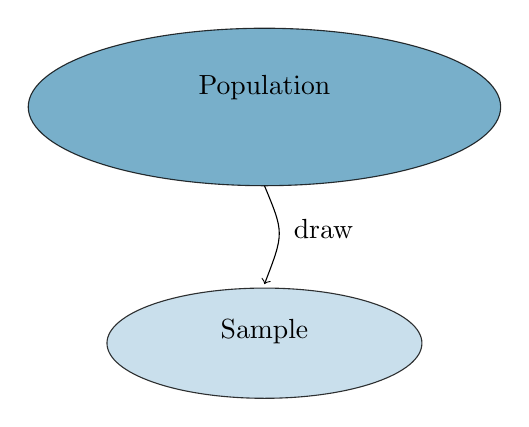
\begin{tikzpicture}
%\draw[style=dashed] (2,.5) circle (0.5);


%\draw[fill=green!30] (1,3)
\draw[fill=oiB, opacity=0.8] (1,3)
ellipse (3 and 1);

\node[draw=none] at (1,3.25) {Population};



\draw[->] (1,2) .. controls (+1.25,1.4) .. (1, 0.75);
\node[draw=none] at (1.750, 1.45) {draw};



%\draw[fill=blue!10] (1,0)
\draw[fill=oiB7, opacity=0.8] (1,0)
ellipse (2 and 0.7);
\node[draw=none] at (1.00, 0.15) {Sample};


%\draw[fill=blue] (0,0) rectangle (1,1);
%\draw[style=thick]
%(3,.5) -- +(30:1) arc(30:80:1) -- cycle;

\end{tikzpicture}
\end{center}


\end{frame}





\subsection*{Introduction to Inferential Statistics Ctd...}

\begin{frame}
\frametitle{Intro to Inferential Statistics Ctd...} 

\vspace{-0.25cm}

\begin{definition}[Parameter]
A numerical measure of a population.
\end{definition}

\begin{itemize}\justifying
\item	Usually \alert{not known} since it is very hard to take measurements on every unit in a population.\\
\hfill\\
\item	Parameters of interest for us:
	\begin{itemize}\justifying
	\item	$\mu$	~:~ Population mean
	\item	$\sigma$	~:~  Population standard deviation
	\item	$p$		~:~  Population proportion
	\end{itemize}
\end{itemize}

\hfill\\


\end{frame}





\subsection*{Introduction to Inferential Statistics Ctd...}

\begin{frame}
\frametitle{Intro to Inferential Statistics Ctd...} 

\begin{definition}[Statistic]
A numerical measure of a sample.
\end{definition}

\begin{itemize}\justifying
\item	\alert{Known} as it is much easier to take measurements on a sample and calculate statistics.\\
\hfill\\
\item	Statistics of interest for us:
	\begin{itemize}\justifying
	\item	$\bar{x}$	~:~ Sample mean
	\item	$s$		~:~ Sample standard deviation
	\item	$\hat{p}$	~:~ Sample proportion
	\end{itemize}
\hfill\\
\vspace{0.2cm}
\item	A statistic is also often referred to as an \alert{estimator}.
\end{itemize}

\hfill\\


\end{frame}







\subsection*{Introduction to Inferential Statistics Ctd...}

\begin{frame}
\frametitle{Intro to Inferential Statistics Ctd...} 

\vspace{-0.50cm}
Updated picture:\\
%\hfill\\

\begin{center}
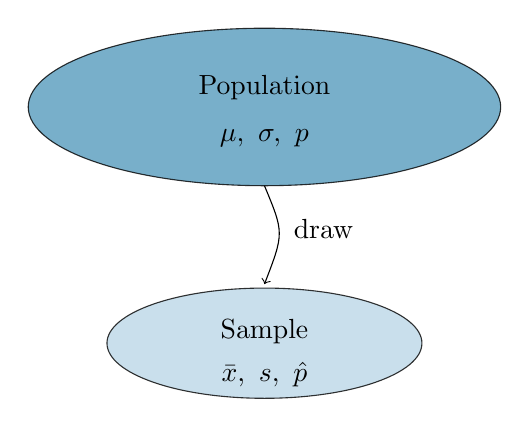
\begin{tikzpicture}
%\draw[style=dashed] (2,.5) circle (0.5);


\draw[fill=oiB, opacity=0.8] (1,3)
ellipse (3 and 1);

\node[draw=none] at (1,3.25) {Population};
\node[draw=none] at (1,2.60) {$\mu, ~\sigma, ~p$};



\draw[->] (1,2) .. controls (+1.25,1.4) .. (1, 0.75);
\node[draw=none] at (1.750, 1.45) {draw};



\draw[fill=oiB7, opacity=0.8] (1,0)
ellipse (2 and 0.7);
\node[draw=none] at (1.00, 0.15) {Sample};
\node[draw=none] at (1,-0.40) {$\bar{x}, ~s, ~\hat{p}$};



%\draw[fill=blue] (0,0) rectangle (1,1);
%\draw[style=thick]
%(3,.5) -- +(30:1) arc(30:80:1) -- cycle;

\end{tikzpicture}
\end{center}


\end{frame}





\subsection*{Introduction to Inferential Statistics Ctd...}

\begin{frame}
\frametitle{Intro to Inferential Statistics Ctd...} 

\begin{goal}[Statistical Inference]
\justifying
To calculate estimators of population parameters, and to quantify the accuracy of these
estimators with probabilities.
\end{goal}
%\hfill\\

%\textcolor<1>{red}{\color<3-4>{blue}text}

\vspace{0.10cm}


\begin{itemize}\justifying
\item	Interested in parameters in a population.\\[0.50em]
% \item	Interested in \textcolor<4-5>{red}{p}arameters in a \textcolor<4-5>{red}{p}opulation.
\item	Calculate statistic from a sample.
%\end{itemize}
\vspace{0.25cm}
\hfill\\
	\begin{center}
	Statistics	 \quad	$\xrightarrow{\text{Estimate}}$	 \quad Parameters
	\end{center}
\hfill\\
\item	Quantify how confident we are about a statistic estimating its corresponding parameter.
\end{itemize}

\end{frame}




\subsection*{Introduction to Inferential Statistics Ctd...}

\begin{frame}
\frametitle{Intro to Inferential Statistics Ctd...} 

\vspace{-0.4cm}
\begin{center}
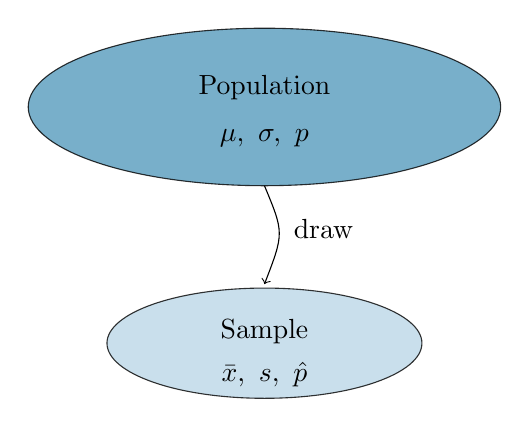
\begin{tikzpicture}
%\draw[style=dashed] (2,.5) circle (0.5);


\draw[fill=oiB, opacity=0.8] (1,3)
ellipse (3 and 1);

\node[draw=none] at (1,3.25) {Population};
\node[draw=none] at (1,2.60) {$\mu, ~\sigma, ~p$};


\draw[->] (1,2) .. controls (+1.25,1.4) .. (1, 0.75);
\node[draw=none] at (1.750, 1.45) {draw};


\draw[fill=oiB7, opacity=0.8] (1,0)
ellipse (2 and 0.7);
\node[draw=none] at (1.00, 0.15) {Sample};
\node[draw=none] at (1,-0.40) {$\bar{x}, ~s, ~\hat{p}$};


\end{tikzpicture}

%\hfill\\

\vspace{0.25cm}

$\bar{x}	\quad	\xrightarrow{\text{Estimate}}	\quad 	\mu$		\\

$s	 	\quad	\xrightarrow{\text{Estimate}}	\quad 	\sigma$	\\

\vspace{0.15cm}
$\hat{p}	\quad	\xrightarrow{\text{Estimate}}	\quad	p$


\end{center}

\end{frame}




\section{Issues with Sample Data}

\subsection*{Introduction}

\begin{frame}
\frametitle{Information on Sample Data} 

\vspace{-0.5cm}

\begin{itemize}\justifying
\item	It is usually very difficult (or impossible) to measure every unit in a population.\\[1.00em]
\item	It is more feasible and practical to draw a sample and take measurements on all units in this sample.\\[1.00em]
\item	We would like our sample to be representative of the population it is drawn from.\\[1.00em]
\item	This is because we would like to make generalizations about the population based on our sample.\\

\vspace{0.25cm}

\begin{center}
Sample	\quad	$\xrightarrow{\text{Generalize}}$ \quad Population
\end{center}
\hfill\\


\end{itemize}

\end{frame}


\subsection*{Types of Samples}

\begin{frame}
\frametitle{Types of samples}

\vspace{-0.50cm}


\begin{definition}[Random Sample]
\justifying
Each unit in a population has an equal chance of being selected.
Also each of combination of size $n$ has an equal chance of selection.
\end{definition}

\vspace{0.25cm}

\begin{itemize}
\item	Other sampling techniques include:
	\begin{itemize}\justifying
	\item	Stratified sampling
	\item	Cluster sampling
	\item	Multistage sampling
	\end{itemize}
\vspace{0.25cm}
\item	However these will not be covered in this course
\end{itemize}

\end{frame}




\subsection*{Issues with Collecting Sample data}

\begin{frame}
\frametitle{Issues with Collecting Sample data}

\footnotesize

\vspace{-1cm}

\begin{itemize}\justifying
\item	Collecting sample data is expensive (in terms of time and money).\\
\item Data may be \alert{biased}:\\
	\hfill\\
%	\vspace{-0.25cm}

	\begin{tabular}{p{2.75cm} p{0.1cm} p{6.5cm}}
	\vspace*{-0.35cm}\alert{Selection bias}		& :	&	 Sample is not representative of the
								population since a subset of the
								population has no chance of being
								selected for the sample			\\[1.0em]					
	\vspace*{-0.35cm}\alert{Nonresponse bias}	& :	&	There may be a reason that certain	
								respondents refuse to participate. As
								such we lose information.				\\[1.0em]
	\vspace*{-0.35cm}\alert{Measurement\newline error bias}	& :	&	The response measured and recorded
									for an individual unit is not correct.		\\	
	\end{tabular}
	\hfill\\
	\vspace{+0.25cm}
\item	Ideally we would like to draw a \alert{random sample}.
\end{itemize}




\end{frame}




\section{Homework}

\subsection*{Homework}

\begin{frame}
\frametitle{Homework}

%\begin{itemize}\justifying
%\item	Custom Edition :	Exercises 1.15 --- 1.17; ~1.25 --- 1.31 \\
%\hfill\\
%\item	11$^{\text{th}}$ Edition :	1.14 --- 1.17; ~1.21 --- 1.28
%\end{itemize}

\vspace{-0.5cm}

\textbf{Readings}

\begin{itemize}\justifying
\item	Introduction to Probability and Statistics\\
	\quad  Read 1.1 --- 1.4.1 (Pages 2 --- 15);\\
	\quad  Read 1.6 (Pages 21 --- 22)
\end{itemize}
\hfill\\
\textbf{Exercises}

\begin{itemize}\justifying
\item	Custom Edition of Statistics for Business and Economics (McClave, Benson, Sincich):\\
	\quad Exercises 1.15 --- 1.17;\\
	\quad Exercises 1.25 --- 1.31 \\
\hfill\\
\item	11$^{\text{th}}$ Edition of Statistics for Business and Economics (McClave, Benson, Sincich):\\
	\quad Exercises 1.14 --- 1.17; \\
	\quad Exercises 1.21 --- 1.28\\
\end{itemize}





\end{frame}



\end{document}